% !TEX root =  ../main_manuscript.tex 
\section{Results}
The cause-specific cumulative upgrading-risk at year five of follow-up was 35\% in PRIAS, and at most 50\% in the five validation cohorts (Panel~B, Figure~\ref{fig:auc_beforecalib}). That is, many patients may not require any biopsy in the first five years of AS.

In the joint model fitted to the PRIAS dataset, the adjusted hazard ratio of upgrading for an increase in patient age from 61 to 71 years (25-th to 75-th percentile) was 1.45~(95\%CI:~1.30--1.63). For an increase in fitted PSA value (log scale) from 2.36 to 3.07 (25-th to 75-th percentile), the adjusted hazard ratio was 0.99~(95\%CI:~0.89--1.11). In contrast to PSA value, instantaneous PSA velocity was a stronger predictor of upgrading-risk, because an increase in velocity from -0.09 to 0.31 (25-th to 75-th percentile) had a hazard ratio of 2.47~(95\%CI:~1.93--2.99). The impact of PSA value and velocity on upgrading-risk varied between cohorts (Table~6, Supplementary~A.2). Detailed results are in Supplementary~A.2.

The time-varying mean absolute risk prediction error; time-varying AUC; and calibration plot of our model in different validation cohorts are shown in Panel~B, Figure~8, Supplementary~B; Panel~A, Figure~\ref{fig:auc_beforecalib}; and Panel~B, Figure~\ref{fig:auc_beforecalib}, respectively. In all cohorts, AUC was moderate (0.55 to 0.75). Mean absolute prediction error was large (0.3 to 0.45) in those cohorts where the impact of PSA value and velocity on upgrading-risk was different from PRIAS (e.g., MUSIC cohort, Table~6, Supplementary~A.2), and moderate (0.1 to 0.3) otherwise. To resolve issues in calibration-at-large (Panel~B, Figure~\ref{fig:auc_beforecalib}), we recalibrated the baseline hazard of upgrading in all cohorts (Figure~6, Supplementary~B). We compared risk predictions from the recalibrated models with predictions from separately fitted joint models to each cohort (Figure~7, Supplementary~B). The difference in predictions was lowest in Johns Hopkins cohort (impact of PSA similar to PRIAS, Table~5, Supplementary~A.2). Comprehensive validation results are in Supplementary~B.

\begin{figure}
\centerline{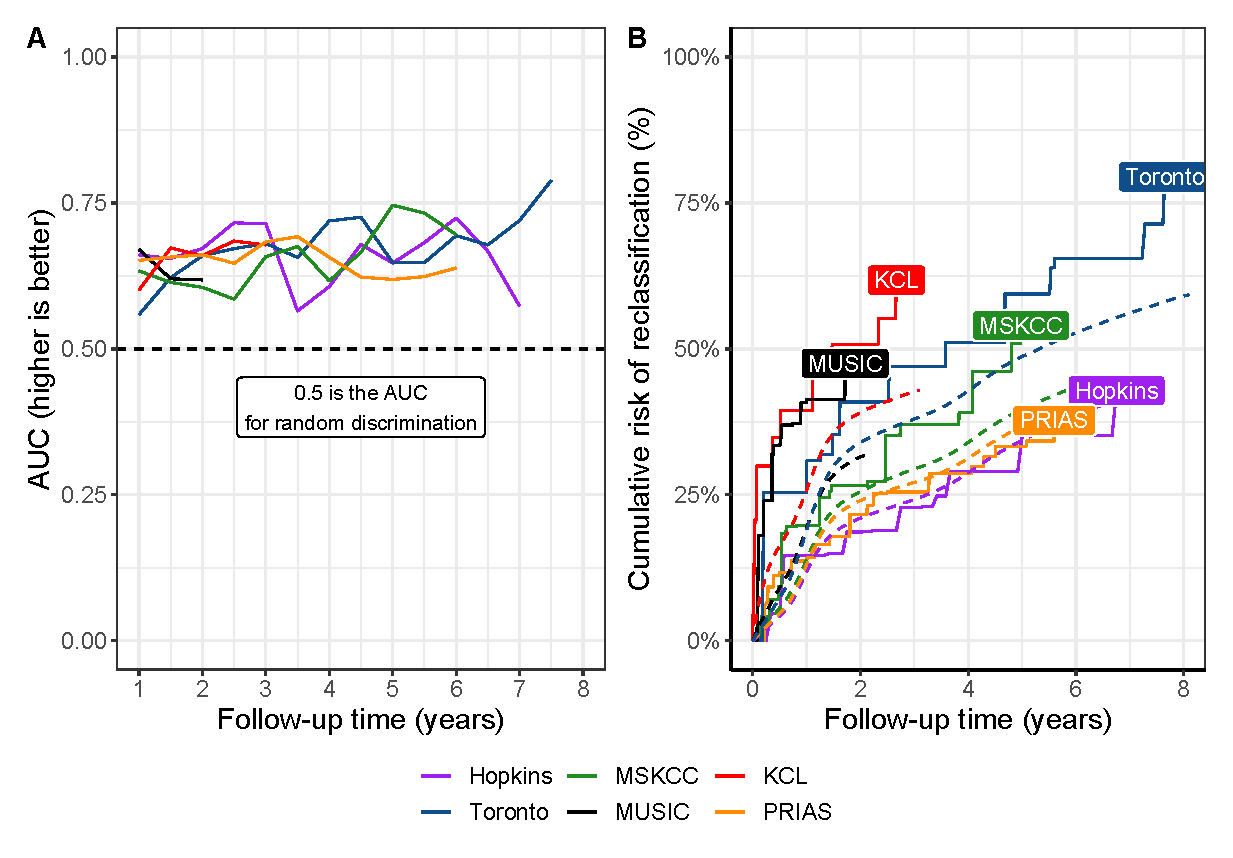
\includegraphics[width=\columnwidth]{images/auc_beforecalib.eps}}
\caption{\textbf{Model Validation Results}. \textbf{Panel~A}: time dependent area under the receiver operating characteristic curve or AUC (measure of discrimination). \textbf{Panel~B}: calibration-at-large indicates model miscalibration. This is because solid lines depicting the non-parameteric estimate of the cause-specific cumulative upgrading-risk~\citep{turnbull1976empirical}, and dashed lines showing the average cause-specific cumulative upgrading-risk obtained using the joint model fitted to the PRIAS dataset, are not overlapping. Same plot after recalibration is shown in Figure~6, Supplementary~B. Full names of Cohorts are \textit{PRIAS}: Prostate Cancer International Active Surveillance, \textit{Toronto}: University of Toronto Active Surveillance, \textit{Hopkins}: Johns Hopkins Active Surveillance, \textit{MSKCC}: Memorial Sloan Kettering Cancer Center Active Surveillance, \textit{KCL}: King's College London Active Surveillance, \textit{MUSIC}: Michigan Urological Surgery Improvement Collaborative Active Surveillance.}
\label{fig:auc_beforecalib}
\end{figure}

\subsection{Personalized Biopsy Schedules}
We utilized the fitted joint model to create upgrading-risk based personalized biopsy schedules. To this end, given a new patient's accumulated PSA measurements (Panel~A,~Figure~\ref{fig:jmExplanationPlot_113}) and biopsy results, we first predicted his cause-specific cumulative upgrading-risk at his current as well as future PSA follow-up visits (Panel~A,~Figure~\ref{fig:demo_pat1}). These PSA visits occur every six months in PRIAS. Subsequently, we scheduled personalized biopsies on those future follow-up visits of a patient, where his conditional cumulative upgrading-risk was more than a certain threshold (Supplementary~C), for example, 10\% risk. We maintained a minimum gap of one year between consecutive biopsies (PRIAS recommendation). Example personalized schedules based on 5\% and 10\% risk thresholds are shown in Panel~B, Figure~\ref{fig:demo_pat1}, and in Figure~9--11, Supplementary~C. Both the risk predictions and resulting personalized schedules were dynamic because they were updated as more follow-up data became available over follow-up (Figure~5, Supplementary~B).

\begin{figure}
\centerline{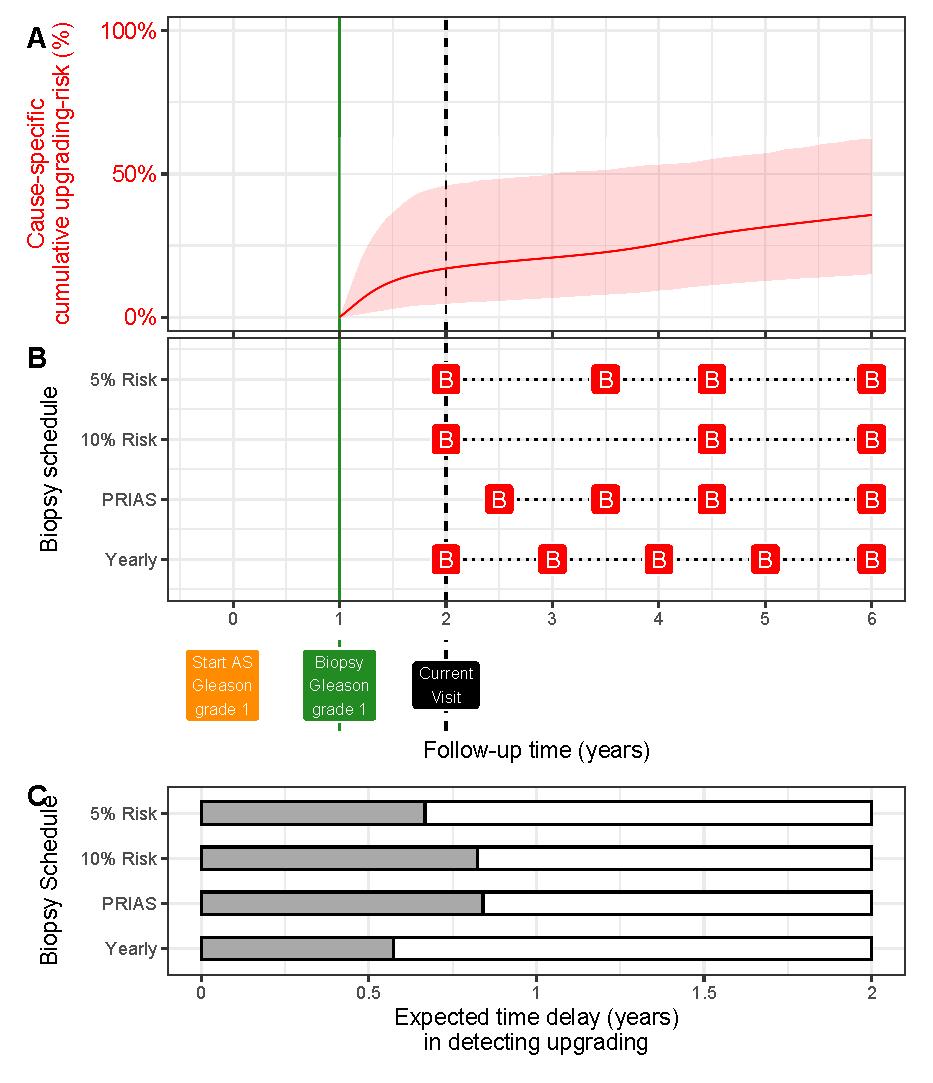
\includegraphics[width=\columnwidth]{images/demo_pat1.eps}}
\caption{\textbf{Illustration of personalized and fixed schedules of biopsies}. Due to a lack of space, the PSA profile of this patient is shown in Figure~\ref{fig:jmExplanationPlot_113}. \textbf{Panel~A:} Predicted cumulative upgrading-risk (95\% credible interval shaded). \textbf{Panel~B:} Personalized and fixed schedules of biopsies, with a red `B' indicating a scheduled biopsy. The green vertical line at year 1 denotes the time of the latest negative biopsy. Black dashed line at year 3 denotes the time of the current visit. \textbf{Panel~C:}\ Expected time delay in detecting upgrading (months) for different schedules. A compulsory biopsy was scheduled at year six (maximum biopsy scheduling time in PRIAS, Supplementary~C) in all schedules for a meaningful comparison between them.}
\label{fig:demo_pat1}
\end{figure}

The choice of the risk threshold in the personalized schedule dictates the timing and the total number of biopsies, and the expected time delay (Figure~\ref{fig:delay_explanation}) in detecting upgrading. We estimated the time delay for both personalized and fixed schedules (Panel~C in Figure~\ref{fig:demo_pat1} and Figure~9--11, Supplementary~C). Since we estimated the time delay in a personalized manner as well, patients/doctors can compare personalized schedules based on different risk thresholds, with fixed schedules, before making a choice.

\subsection{Web-Application}
We implemented our model and personalized schedules in a user-friendly web-application \url{https://emcbiostatistics.shinyapps.io/prias_biopsy_recommender/}. Currently, the web-application supports PRIAS and the five validation cohorts. Patient data can be entered manually and in Microsoft Excel format. Predictions for upgrading-risk are available for a currently limited, cohort-specific, follow-up period (Table 7, Supplementary~C). The web-application visualizes the timing of biopsies, and expected time delay in detecting upgrading, for personalized schedules based on 5\%, 10\%, and 15\% risk threshold; annual biopsies; biennial biopsies; and PRIAS schedule.